\section{Results}\label{sec:results}

\subsection{Performance depends on the endpoint, not on the model class}\label{subsec:cross-task-results}

The best model depended on the task (Tables~\ref{tab:baselines-regression} and \ref{tab:baselines-classification}). The descriptor MLP and the framework direct hybrid tied for the lowest mean RMSE on ESOL ($0.623$), the framework direct hybrid was best on Lipophilicity ($0.606$), and Chemprop's D-MPNN with descriptors was best on FreeSolv ($0.946$) and BBBP ($0.923$); the RDKit 2D Random Forest remained best on BACE ($0.822$). After Holm correction only two paired comparisons excluded zero: the framework hybrid beat the RDKit 2D Random Forest on Lipophilicity ($\Delta=-0.142$, corrected 95\% CI $[-0.179,-0.106]$, 10/10 splits) and trailed it on BACE (hybrid $-0.037$ AUROC, $[-0.058,-0.017]$, 0/10 wins); every other comparison was inconclusive, including the ESOL hybrid-versus-Random-Forest and hybrid-versus-graph-only contrasts (Additional file 1, Table S8). Descriptors outperformed ECFP4 fingerprints with Random Forests on every task, although the BACE margin was negligible ($0.822$ versus $0.822$ at the displayed precision).

\begin{table}[t]
\caption{Regression performance (RMSE, mean $\pm$ SD over ten saved splits). Bold marks the best mean in each column; ties at the displayed precision are both bold.}
\label{tab:baselines-regression}
\centering
\footnotesize
\setlength{\tabcolsep}{4pt}
\begin{tabular}{@{}lccc@{}}
\toprule
Model & ESOL & FreeSolv & Lipophilicity \\
\midrule
\multicolumn{4}{@{}l}{\emph{Reference models}} \\
Dummy & $1.894\pm0.197$ & $3.619\pm0.388$ & $1.148\pm0.039$ \\
ECFP4 + Random Forest & $1.352\pm0.093$ & $1.795\pm0.306$ & $0.853\pm0.028$ \\
RDKit 2D + Random Forest & $0.637\pm0.061$ & $1.089\pm0.175$ & $0.748\pm0.025$ \\
Descriptor MLP & $\mathbf{0.623\pm0.040}$ & $1.290\pm0.446$ & $0.683\pm0.023$ \\
\midrule
\multicolumn{4}{@{}l}{\emph{Chemprop v2.3.1}} \\
Graph-only D-MPNN & $0.791\pm0.063$ & $1.178\pm0.320$ & $0.641\pm0.085$ \\
D-MPNN + descriptors ($x_d$) & $0.844\pm0.640$ & $\mathbf{0.946\pm0.261}$ & $0.639\pm0.068$ \\
\midrule
\multicolumn{4}{@{}l}{\emph{Framework}} \\
Graph only (\cfg{residual\_only}) & $0.623\pm0.092$ & $1.251\pm0.153$ & $0.607\pm0.031$ \\
Graph + descriptors (\cfg{direct\_hybrid}) & $\mathbf{0.623\pm0.054}$ & $1.099\pm0.249$ & $\mathbf{0.606\pm0.019}$ \\
Prior + graph residual (\cfg{prior\_residual}) & $0.681\pm0.113$ & $1.175\pm0.207$ & $0.609\pm0.036$ \\
\bottomrule
\end{tabular}
\end{table}

\begin{table}[t]
\caption{Classification performance (AUROC, mean $\pm$ SD over ten saved splits). Bold marks the best mean in each column; ties at the displayed precision are both bold.}
\label{tab:baselines-classification}
\centering
\footnotesize
\setlength{\tabcolsep}{5pt}
\begin{tabular}{@{}lcc@{}}
\toprule
Model & BBBP & BACE \\
\midrule
\multicolumn{3}{@{}l}{\emph{Reference models}} \\
Dummy & $0.500\pm0.000$ & $0.500\pm0.000$ \\
ECFP4 + Random Forest & $0.905\pm0.022$ & $0.822\pm0.028$ \\
RDKit 2D + Random Forest & $0.912\pm0.019$ & $\mathbf{0.822\pm0.027}$ \\
Descriptor MLP & $0.915\pm0.028$ & $0.787\pm0.034$ \\
\midrule
\multicolumn{3}{@{}l}{\emph{Chemprop v2.3.1}} \\
Graph-only D-MPNN & $0.911\pm0.024$ & $0.808\pm0.056$ \\
D-MPNN + descriptors ($x_d$) & $\mathbf{0.923\pm0.019}$ & $0.793\pm0.040$ \\
\midrule
\multicolumn{3}{@{}l}{\emph{Framework}} \\
Graph only (\cfg{residual\_only}) & $0.914\pm0.034$ & $0.802\pm0.038$ \\
Graph + descriptors (\cfg{direct\_hybrid}) & $0.916\pm0.029$ & $0.785\pm0.033$ \\
Prior + graph residual (\cfg{prior\_residual}) & $0.910\pm0.034$ & $0.783\pm0.062$ \\
\bottomrule
\end{tabular}
\end{table}

The framework and Chemprop graph only models were close: the framework was more accurate on ESOL ($0.623$ versus $0.791$, nominal $p=0.027$, Holm-adjusted $p=0.053$ within the two external comparisons for that dataset), Chemprop was more accurate on FreeSolv ($1.252$ versus $1.178$, not significant), and the remaining tasks were indistinguishable; across tasks the framework won between three and nine of ten splits (Additional file 1, Table S9). More informative than either ranking was the effect of adding descriptors (Fig.~\ref{fig:descriptor-effect}). In the framework the change in the mean was small on ESOL ($+0.1\%$), Lipophilicity ($+0.1\%$) and BBBP ($+0.2\%$), clearly positive on FreeSolv ($+12.1\%$), and slightly negative on BACE ($-2.1\%$). Chemprop showed the same pattern on FreeSolv ($+19.7\%$), Lipophilicity ($+0.2\%$), BBBP ($+1.3\%$) and BACE ($-1.9\%$), but on ESOL its descriptor hybrid was better on nine of the ten splits and failed badly on one (test RMSE $2.76$), so the mean fell by $6.8\%$ with an SD of $0.64$. That failure is diagnosed in Section~\ref{subsec:divergence-results}: retraining the same configuration on that split with six seeds spans $0.75$ to $6.12$ RMSE, so the mean over one seed per split is not an estimate of a stable effect and its sign on ESOL is not interpreted. Reporting only that mean would have reversed the sign of the effect on ESOL, and the per-split record kept by the workflow is what makes the instability visible. On the four endpoints without such a failure the two implementations agreed on the sign and approximate size of the descriptor effect, which suggests that the effect is a property of the task and protocol rather than of the code.

\begin{figure}[t]
\centering
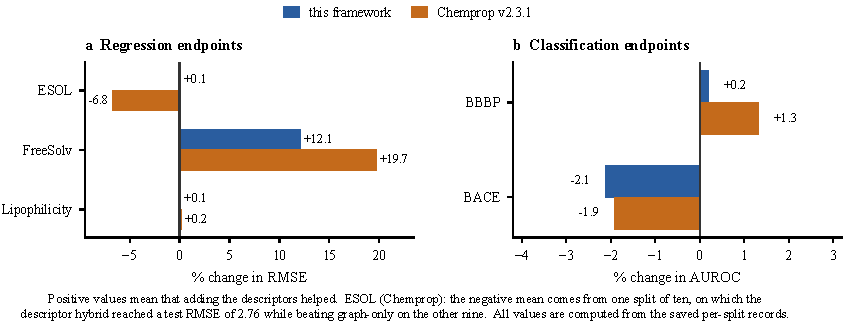
\includegraphics[width=150mm]{figs/fig3_descriptor_effect.pdf}
\caption{Effect of adding 210 RDKit descriptors to a graph-only D-MPNN, in two independently written implementations. Panel (a) shows regression endpoints and panel (b) classification endpoints, so the two metric families are not mixed on one axis. Bars are the change in the ten-split mean of the primary metric (RMSE in (a), AUROC in (b)), signed so that positive values mean lower error or higher AUROC. The ESOL value for Chemprop is dominated by one split, in which its descriptor hybrid reached a test RMSE of 2.76 while being better than graph-only on the other nine; retraining that configuration on that split with six seeds spans 0.75 to 6.12 RMSE, and bounding the descriptor inputs collapses the six retrainings to 0.65--0.72, so the ESOL bar is not an estimate of a stable effect. Computed from Tables~\ref{tab:baselines-regression} and \ref{tab:baselines-classification}.}
\label{fig:descriptor-effect}
\end{figure}

\subsection{Descriptor evidence shows what the data support, not what is universally important}\label{subsec:feature-results}

A chemist approaching a new endpoint asks two things before any model is trained: are the records trustworthy, and which of the several hundred descriptors are actually supported by the training molecules? The audit answers the first, the scorecard and the selectors answer the second, and the two answers are independent of the learner. The audit found duplicated structures in two of the five benchmarks (Table~\ref{tab:hygiene}, discussed below).

Figure~\ref{fig:worked} follows a single molecule through both checks, so that the numbers in the tables can be read on a concrete case.

\begin{figure}[t]
\centering
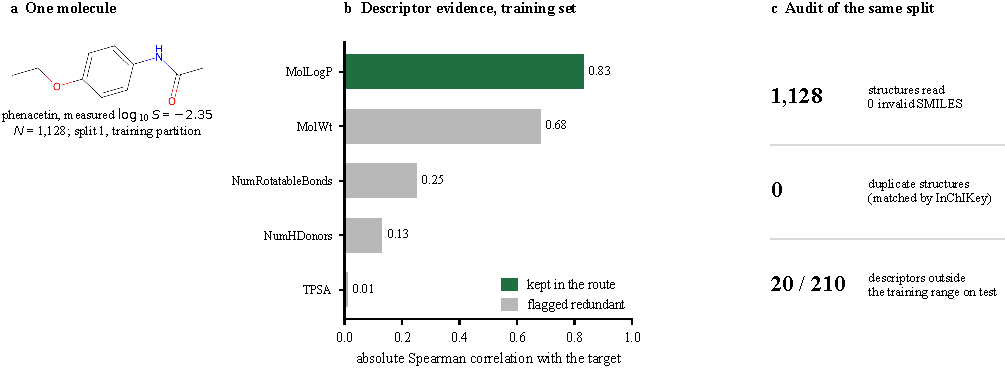
\includegraphics[width=\textwidth]{figs/fig2_worked_example.pdf}
\caption{One molecule followed through the audit and the descriptor scorecard. (a) Phenacetin in the ESOL dataset; its measured aqueous solubility is $\log_{10}S=-2.35$ and it belongs to the training partition of split 1. (b) Training-partition evidence for five of the 210 descriptors. Bars are absolute Spearman correlations with the measured solubility; a descriptor is grey if the recommender did not keep it, which in these cases is because its Pearson correlation with a higher-ranked descriptor exceeded 0.85. (c) Audit output for the same split. The full scorecard covers every descriptor and every split.}
\label{fig:worked}
\end{figure}

With a Random Forest as learner (ESOL, FreeSolv, BBBP), recommended subsets had better mean scores than random subsets of the same size at every budget, and the corrected intervals excluded zero at all budgets on ESOL, at $K\leq20$ on FreeSolv, and at $K=5$ on BBBP; the margin shrank as $K$ grew. At $K=50$ on ESOL, 10 and 20 on FreeSolv, and the three larger budgets on BBBP, the recommendation still had the better mean but the corrected interval did not separate it from random draws. Against the full 210-descriptor pool the picture reverses: at $K=5$ and $K=10$ on ESOL the recommended subset was significantly worse, and every other budget was inconclusive (Additional file 1, Table S4).

A ten-draw control carries its own draw noise, so the comparison was repeated with 50 draws per split and budget in all five endpoints, keeping every draw and testing the recommendation's rank inside the resulting distribution (Additional file 1, Table S5). The recommended subset had the better mean in all 20 dataset--budget cells, and the Fisher-combined rank test was significant in 16: all twelve regression cells ($p\leq1.1\times10^{-3}$; mean percentile $0.88$--$1.00$) and four of the eight classification cells (BBBP at $K=5,10,20$ and BACE at $K=5$, $p=4.4\times10^{-4}$ to $0.036$). The four that did not separate are the larger classification budgets (BBBP $K=50$ and BACE $K=10,20,50$), where a Random Forest on any 50 descriptors already approaches the full-pool AUROC: on BBBP the 50-draw mean is $0.774$ at $K=5$ but $0.905$ at $K=50$, against $0.916$ for the full pool. The advantage of the evidence-based subset is therefore systematic, and largest where descriptors are scarce; it is not a claim that 50 chosen descriptors beat 50 random ones on a classification endpoint.

Across six selectors on five datasets (Table~\ref{tab:selectors}), Random Forest importance and mutual information ranked best on average, with mean ranks of 2.20 and 2.35, respectively. The framework recommender ranked fourth (3.65), was best in one of the 20 dataset-budget cells, and had mean pairwise Jaccard stability of 0.76. This stability was below Spearman ranking (0.88) and mutual information (0.80), but above Random Forest importance (0.65), MI--Pearson (0.57), and L1 (0.47). A Friedman test over the 20 dataset-budget cells rejects equality of the six selectors ($\chi^2=38.3$, $p=3.3\times10^{-7}$), but after Nemenyi correction at $\alpha=0.05$ (critical difference 1.69 ranks) the recommender is not separated from any individual selector, including the best: its gap to Random Forest importance is 1.45 ranks. The individual selector comparisons that survive Holm correction within a dataset are listed in Additional file 1, Table S7. These results support a transparent and reasonably stable candidate-generation heuristic, not a selector that consistently outperforms established alternatives. The selector match with the downstream Random Forest may favour RF importance. Read against the three criteria stated for H1, the 50-draw control meets (i) in all 20 cells on the mean comparison and in 16 on the rank test, the selector comparison fails (ii), and the stability analysis meets (iii).

The practical reading for a chemist is therefore: the scorecard tells you what the data can support, the recommender proposes a compact and stable subset, and the ranking among selectors is close enough that the choice should be made on inspectability and stability rather than on a small score difference.

\begin{table}[t]
\caption{Six feature selectors on five datasets with a Random Forest downstream. Mean rank (1 = best) per dataset over $K\in\{5,10,20,50\}$ and overall over 20 dataset-budget cells; Best denotes cells in which the selector had the best mean score; Jaccard: mean pairwise stability over splits and cells. Full results in Additional file 1, Table S6.}
\label{tab:selectors}
\centering
\footnotesize
\setlength{\tabcolsep}{4pt}
\begin{tabular}{@{}lcccccccc@{}}
\toprule
 & \multicolumn{5}{c}{Mean rank per dataset} & & & \\
\cmidrule(lr){2-6}
Selector & ESOL & FreeSolv & Lipo. & BBBP & BACE & Overall & Best & Jaccard \\
\midrule
RF impurity importance & 1.0 & 1.8 & 1.8 & 4.8 & 1.8 & 2.20 & 10 & 0.65 \\
Mutual information & 2.8 & 2.5 & 1.5 & 2.2 & 2.8 & 2.35 & 3 & 0.80 \\
MI-Pearson & 3.8 & 4.2 & 3.5 & 1.5 & 2.8 & 3.15 & 4 & 0.57 \\
Framework recommender & 3.8 & 3.2 & 3.5 & 3.8 & 4.0 & 3.65 & 1 & 0.76 \\
Spearman top-$K$ & 3.8 & 3.2 & 5.0 & 5.8 & 5.8 & 4.70 & 0 & 0.88 \\
L1 (lasso / L1-logistic) & 6.0 & 6.0 & 5.8 & 3.0 & 4.0 & 4.95 & 2 & 0.47 \\
\bottomrule
\end{tabular}
\end{table}

\subsection{The data audit finds problems that the training score cannot see}\label{subsec:audit-results}

The audit found duplicated structures in two of the five benchmarks (Table~\ref{tab:hygiene}). BBBP contained 64 structures recorded more than once (132 records, 6.5\%), 11 of them with conflicting labels; ESOL contained 11 duplicated structures whose label spans stayed below the conflict threshold (largest span 1.03 log units, compared with a threshold of 1.0478). Across the ten scaffold splits, the mean number of out-of-range descriptors was $19.4\pm12.8$ for ESOL, $20.8\pm14.8$ for Lipophilicity, and $15.1\pm9.5$ for BBBP; the corresponding fractions of test molecules affected were $6.3\pm2.5\%$, $3.7\pm0.7\%$, and $3.8\pm2.1\%$, respectively. These diagnostics are range-based indicators rather than a comprehensive measure of distribution shift. In BBBP the relationship was not monotone: the hybrid's weakest split (split 8) had 19 out-of-range descriptors and 8.8\% of test molecules affected, but split 3 had almost as many (18) and gave the hybrid its best score (Additional file 1, Table S3). A range-based count is therefore a warning flag, not a predictor of which split will be hardest.

\begin{table}[t]
\caption{Structure-level audit by InChIKey. Duplicated structures are structures recorded more than once (records in parentheses). Conflicts are duplicated structures whose labels disagree (classification) or span more than half the target standard deviation (regression).}
\label{tab:hygiene}
\centering
\footnotesize
\begin{tabular}{@{}lrrrrr@{}}
\toprule
Dataset & Records & Unique InChIKeys & Duplicated structures & Conflicts & Largest span \\
\midrule
ESOL & 1,128 & 1,117 & 11 (22) & 0 & 1.03 \\
FreeSolv & 642 & 642 & 0 (0) & 0 & 0.00 \\
Lipophilicity & 4,200 & 4,200 & 0 (0) & 0 & 0.00 \\
BBBP & 2,039 & 1,971 & 64 (132) & 11 & -- \\
BACE & 1,513 & 1,513 & 0 (0) & 0 & -- \\
\bottomrule
\end{tabular}
\end{table}

The duplicate-controlled BBBP sensitivity analysis retained 1,960 unique structures after excluding the 11 conflicting label groups and retaining one record for each of the 53 remaining duplicated groups. On ten new scaffold manifests, mean AUROC was $0.8656\pm0.0577$ for the framework graph only model and $0.8637\pm0.0422$ for its descriptor hybrid. Chemprop v2.3.1 achieved $0.8686\pm0.0398$ with graph only and $0.8744\pm0.0428$ with the 210 molecular descriptors, while RDKit 2D plus Random Forest achieved $0.8940\pm0.0305$ (Additional file 1, Table S16). The hybrid minus graph mean difference was $-0.0019$ for the framework (5/10 splits favoured the hybrid) and $+0.0057$ for Chemprop (9/10 splits favoured the hybrid). For the framework the paired 95\% $t$ interval included zero, so these results do not establish a conclusive advantage from descriptor augmentation in this workflow. The Chemprop hybrid-minus-graph difference was in the same direction but smaller, and its interval also included zero; after Holm correction within the five sensitivity comparisons neither implementation separates (Additional file 1, Table S17). The exact ranking differed from the primary benchmark. Scores were lower for the learned models on the sensitivity data, but this change cannot be attributed to duplicate leakage alone because both data composition and split manifests differed.

\subsection{Descriptor routing depends on feature budget and endpoint}\label{subsec:routing-results}

The harmonised routing results show that the value of a compact descriptor route depends on the endpoint (Table~\ref{tab:routing}). The full 210-descriptor hybrid had the lowest mean RMSE on ESOL ($0.614\pm0.039$) and FreeSolv ($1.038\pm0.214$). On Lipophilicity the recommender route had the lowest mean of the six routes ($0.581\pm0.041$), below the full descriptor set ($0.606$); on BACE the graph-only model had the highest mean AUROC ($0.798$), and the six routes spanned only $0.014$, less than the between-split SD. On BBBP every route lay within $0.007$ AUROC of the best. The random-subset control is the important comparator. The recommender beat it on Lipophilicity ($0.581$ versus $0.591$), but was within one SD of it on ESOL ($0.620$ versus $0.631$), FreeSolv ($1.147$ versus $1.149$), BBBP ($0.915$ versus $0.910$) and BACE ($0.797$ versus $0.792$), and every paired recommender-minus-control difference had a Holm-corrected interval that included zero (Additional file~1, Table~S11). The same correction left the Lipophilicity gap to the full descriptor set inconclusive, so the apparent benefit of compactness is not established at this sample size either. A compact route therefore does not appear to require an informed selection rule on these endpoints; what matters is that it is tested rather than assumed. Per-split outputs and checkpoint decisions are archived in the repository; the checkpoint selection rule and result-file inventory are documented in Additional file~1, Table~S18.

\begin{figure}[t]
\centering
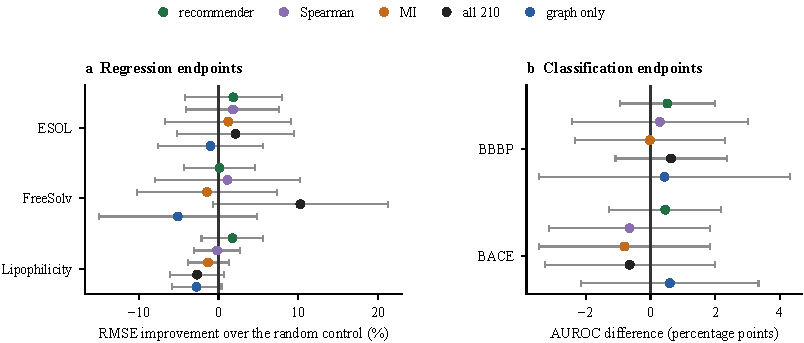
\includegraphics[width=0.92\textwidth]{figs/fig4_routing.pdf}
\caption{Compact descriptor routes compared with the matched random control. Points are mean paired differences over ten splits and error bars are population SDs. Positive values mean that the route had a lower RMSE (a) or a higher AUROC (b) than a random subset of the same size drawn at the same split-specific budget $K^*$. The largest mean improvement is the full descriptor set on FreeSolv (about 10\%), but every interval includes zero: at this sample size no route is separated from its control.}
\label{fig:routing}
\end{figure}

\begin{table}[t]
\caption{Harmonised evidence-guided descriptor routing. Entries are test RMSE for ESOL, FreeSolv, and Lipophilicity, and test AUROC for BBBP and BACE; values are mean $\pm$ population SD over ten saved splits. All route checkpoints are selected by minimum validation loss, and the recommended route's $K^*$ is selected using the primary validation metric at that checkpoint. The random route averages ten random-subset draws per split. Bold text marks the best mean in each row. The two univariate selectors (Spearman and mutual information) are reported in Additional file 1, Table S10, together with the full checkpoint-level audit of 250 model runs (Table S18).}
\label{tab:routing}
\centering
\footnotesize
\setlength{\tabcolsep}{3.2pt}
\begin{tabular}{@{}llcccc@{}}
\toprule
Dataset & Metric & Graph only & All 210 & Recommender & Random \\
ESOL & RMSE $\downarrow$ & $0.638\pm0.074$ & $\mathbf{0.614\pm0.039}$ & $0.620\pm0.078$ & $0.631\pm0.057$ \\
FreeSolv & RMSE $\downarrow$ & $1.205\pm0.164$ & $\mathbf{1.038\pm0.214}$ & $1.147\pm0.140$ & $1.149\pm0.141$ \\
Lipophilicity & RMSE $\downarrow$ & $0.607\pm0.031$ & $0.606\pm0.019$ & $\mathbf{0.581\pm0.041}$ & $0.591\pm0.027$ \\
BBBP & AUROC $\uparrow$ & $0.914\pm0.034$ & $\mathbf{0.916\pm0.029}$ & $0.915\pm0.023$ & $0.910\pm0.020$ \\
BACE & AUROC $\uparrow$ & $\mathbf{0.798\pm0.038}$ & $0.786\pm0.033$ & $0.797\pm0.036$ & $0.792\pm0.042$ \\
\bottomrule
\end{tabular}
\end{table}

\subsection{Configurable predictive roles are useful but not uniformly beneficial}\label{subsec:modularity-results}

The best role assignment was also task dependent (Table~\ref{tab:ablation}). The descriptor-only role was best on ESOL ($0.619$), direct fusion on FreeSolv, Lipophilicity, and BBBP, and graph only on BACE ($0.802$ versus $0.785$ for direct fusion). The margins were often small: on Lipophilicity and ESOL the four learned roles other than the prior and prior-plus-residual variants spanned $0.004$ and $0.018$ RMSE respectively, so the ordering should be read as a trend across ten splits rather than as a separated ranking. No paired interval excluded zero for the prior/residual model against graph only on any task, and on ESOL it had the largest split-to-split variability of the learned models. At the level of training seeds, variation was small relative to split variation for most models (SD over three seeds 0.003 - 0.007 AUROC on BBBP), but reached 0.013 for the prior/residual model, about a third of its between-split SD of 0.034 (Additional file 1, Table S12).

\begin{table}[t]
\caption{Predictive-role ablation (primary metric, mean $\pm$ SD over ten splits; RMSE for ESOL, FreeSolv, and Lipophilicity, AUROC for BBBP and BACE). Bold text marks the best mean per column.}
\label{tab:ablation}
\centering
\footnotesize
\setlength{\tabcolsep}{3pt}
\begin{tabular}{@{}lccccc@{}}
\toprule
Configuration & ESOL & FreeSolv & Lipophilicity & BBBP & BACE \\
\midrule
\cfg{prior\_only} & $0.913\pm0.073$ & $2.015\pm0.116$ & $1.009\pm0.036$ & $0.812\pm0.030$ & $0.660\pm0.055$ \\
\cfg{direct\_only} & $\mathbf{0.619\pm0.045}$ & $1.350\pm0.458$ & $0.683\pm0.034$ & $0.903\pm0.041$ & $0.785\pm0.046$ \\
\cfg{residual\_only} & $0.623\pm0.092$ & $1.251\pm0.153$ & $0.607\pm0.031$ & $0.914\pm0.034$ & $\mathbf{0.802\pm0.038}$ \\
\cfg{direct\_hybrid} & $0.623\pm0.054$ & $\mathbf{1.099\pm0.249}$ & $\mathbf{0.606\pm0.019}$ & $\mathbf{0.916\pm0.029}$ & $0.785\pm0.033$ \\
\cfg{prior\_residual} & $0.681\pm0.113$ & $1.175\pm0.207$ & $0.609\pm0.036$ & $0.910\pm0.034$ & $0.783\pm0.062$ \\
\bottomrule
\end{tabular}
\end{table}

\subsection{Robustness of the inferences}\label{subsec:robustness-results}

Four checks asked whether the conclusions survive a change of statistical view, a change of control protocol, a change of two conventions, and a change of environment.

The primary interval is a Nadeau--Bengio corrected resampled $t$ interval, which is conservative when training sets overlap. Repeating all 184 paired comparisons with an exact sign-flip permutation test, which is computationally exact but makes no overlap correction and is therefore more permissive, reached the same decision in 175 of 184 comparisons and found 23 significant differences rather than 14. The nine disagreements all involve effects whose intervals barely include or exclude zero; none changes a direction, so the conclusions are unchanged when the stricter corrected-interval view is used (Additional file 1, Table S19).

For the routing experiment, none of the 15 route-versus-control comparisons reached significance under the permutation test either (Holm-adjusted $p=1.000$ throughout), so the finding that compact routes are not reliably better than random subsets of the same size does not depend on the interval used.

Two conventions were also varied rather than assumed. Changing the redundancy threshold of the recommender over $0.70$--$0.90$ moved the selected set substantially (mean Jaccard $0.51$--$0.77$ against the default) but changed its downstream score by at most $0.024$ RMSE on ESOL, $0.015$ on FreeSolv and $0.005$ AUROC on BBBP; changing the encoder width over $64$--$256$ kept the sign of the descriptor effect on FreeSolv and changed its size between $7\%$ and $19\%$ (Additional file 1, Tables S20 and S21). In both cases the convention was not what the conclusion depended on.

Finally, because the framework and the Chemprop comparator ran in separate environments with different RDKit releases, the 210-column descriptor block was exported from both and compared cell by cell: 99.87\% of 1{,}999{,}620 cells agree. The differences are confined to ten descriptors, mostly functional-group counts, and are the reason the cross-implementation comparison is described as a replication rather than as an identical-input ablation.

\subsection{The divergent run, diagnosed}\label{subsec:divergence-results}

Two runs in the study departed from every other run of the same configuration, both on ESOL split 3: Chemprop's descriptor hybrid reached a test RMSE of $2.76$ while being better than graph-only on the other nine splits, and the framework's prior/residual route reached $13.23$. Excluding them would have been a post-hoc decision, so both were investigated instead.

Retraining the framework route with three independent training seeds reproduced the failure in all three runs ($13.24$, $13.25$, $13.22$), whereas the direct hybrid on the same split, descriptors and budget gave $0.707$, $0.693$ and $0.727$. The failure is therefore a property of the route and the split, not of one optimisation trajectory. The mechanism is visible in the predicted values: the ridge prior, fitted on the same 50 descriptors, produced test predictions between $-8.09$ and $128.72$ for targets between $-8.40$ and $1.58$, and the residual head adds only a small correction on top of that.

The cause is a single descriptor. \cfg{Ipc} (information content) has a training mean of $2.33\times10^{5}$ and a training SD of $1.70\times10^{6}$ on this split, and the split-3 test set contains a molecule with $\mathrm{Ipc}=5.29\times10^{9}$, which is $3114$ training SDs from the mean. The harness standardises descriptors and replaces infinities by $\pm3$, but it does not bound large finite values, so the network and the ridge prior receive an input of $3113.7$; the largest standardised test value on the other nine ESOL splits is $30.0$. The nonlinear hybrid encoder absorbs this because its descriptor branch is normalised after the first linear layer; the prior/residual route does not, because it adds a linear prediction directly.

Chemprop's hybrid is less stable on the same split. Retraining its archived configuration with six seeds, holding the split, the descriptor block, the model and every hyperparameter fixed, gives test RMSE $0.75$, $1.01$, $1.20$, $2.33$, $5.40$ and $6.12$, with maximum absolute predictions of $8.2$, $9.7$, $12.2$, $24.7$, $50.2$ and $57.2$ against targets spanning $-8.40$ to $1.58$. The archived value of $2.76$ is therefore one draw from an unstable configuration rather than a unique accident: three of the six retrained runs exceed $2.0$ and three stay below $1.3$. Because the archived study trained one seed per split, the Chemprop ESOL descriptor effect of $-6.8\%$ is a property of the seed used on split 3, and we do not interpret its sign; the within-system framework contrast for the same endpoint, which is stable across splits, puts the effect at approximately zero.

The intervention confirms the mechanism. Winsorising the standardised descriptor block at $\pm5$ training standard deviations, with the data, split, model, seeds and all other hyperparameters unchanged, gives $0.666$, $0.699$, $0.719$, $0.698$, $0.653$ and $0.677$ RMSE for the same six seeds: a spread of $0.066$ instead of $5.37$, and a mean of $0.685$ against $2.802$ without the bound. Bounding the magnitude of the descriptor inputs, and nothing else, therefore removes both the tail and the instability. The stabilised hybrid is also close to the graph-only arm on the same split ($0.673$), so once the input is bounded the ESOL descriptor effect is approximately zero rather than negative; the framework's within-system contrast reaches the same conclusion ($+0.1\%$). The failure is a property of the input magnitude, not of Chemprop's training procedure.

The range audit had already flagged the split: ESOL split 3 has 44 of 210 descriptors outside the training range and $11.5\%$ of test molecules affected, more than any other ESOL split. The aggregate count was not sufficient, however, because it does not separate a descriptor one unit beyond the training range from one $3114$ standard deviations beyond it, and Lipophilicity split 9 has more out-of-range descriptors (60) with no divergence. Magnitude separates them: the largest standardised test value on ESOL split 3 is $3114$, against at most $30.0$ on the other nine ESOL splits and at most $62$ on the Lipophilicity splits; the only comparably large values in the audit are BBBP splits 6 and 8 ($430$ and $478$, both on \cfg{Kappa3}), where nothing diverged. A maximum-magnitude check is therefore a warning to inspect rather than a verdict, and we report it in the audit output alongside the range count, with values in the hundreds of training standard deviations treated as a reason to winsorise the descriptor block before interpreting the score.


